\documentclass{article}

\usepackage{tikz}
\usepackage{amsfonts}
\usepackage{amssymb}
\usepackage{mathtools}

\usepackage[english]{babel}
\usepackage[autostyle]{csquotes}
\MakeOuterQuote{"}

\title{The Calculus of Constructions, EliDupree Edition}
\author{Eli Dupree}
\date{\today}

\newcommand{\Prop}{\mathbb{P}}
\newcommand{\istype}{\ \mathrm{type}}
\newcommand{\usage}{\mathcal{V}}
\newcommand{\usageKnown}[2]{\usage\{#2:#1\}}
\newcommand{\presep}{\hspace{1.8em}}
\newcommand{\subst}[3]{#1[{#2}{/}{#3}]}
\newcommand{\subty}[1]{#1^*}
\newcommand{\bindvariable}{\bigstar}
\newcommand{\bindnotthis}{\circ}
\newcommand{\emptybindingslike}[1]{\varnothing #1}
\newcommand{\betaeq}{\overset{\beta}{=}}
\newcommand{\betared}[1]{\overset{#1}{\rightarrow}}

\begin{document}
  \maketitle

  \section{Fundamentals}
  \subsection{Formulas}

  The Calculus of Constructions (CoC) is a system of formulas. The following context-free grammar shows the six elementary "formula constructors" – ways to build a formula, sometimes from smaller formulas ($F$):

  \[ F \rightarrow \Prop \mid \usage \mid \usageKnown{F}{F} \mid \lambda b:F,F \mid \forall b:F,F \mid (F F) \]
  
  By combining these constructors into larger formulas, you can express all of computation and mathematics. Our definitions are mainly concerned with judging which of these formulas are \textbf{types}, and which other formulas are \textbf{members} of those types. Anywhere you see the symbol $:$, as in $v : T$, it means a claim that something is a member of the type $T$.

  Here is an informal description of each formula constructor:

  $\Prop$ (read as "Prop") is the \emph{type of all ordinary types}. It's called "Prop" because the ordinary types can represent \emph{propositions} (although they can represent many other things as well).
  
  $\lambda b:T,v$ ("a lambda") is a \emph{function} which maps a single parameter, of type $T$, to the formula $v$ (after the value of the parameter is substituted into $v$) We call $T$ the \textbf{parameter type}, and $v$ the \textbf{body} or \textbf{return value}.
  
  $\forall b:T,U$ ("a forall", read as "for all $b$ in $T$, $U$") is the \emph{type} of any $\lambda c:T,v$ where $v : U$. We call these types "foralls" because of the way that types can represent propositions: The members of a type are the proofs of a proposition, and a proposition with no proofs (an empty type) is a false proposition\footnote{A fan of Gödel might ask: "What about propositions that are true but unprovable?" Well, we are free to define "true" to mean "provable within CoC". We are speaking of \emph{constructive} truth, which is a slightly stronger claim than truth in classical logic. Like all theories, CoC must be incomplete, but the form of that incompleteness is just that there are some propositions $P$ where neither $P$ nor $\neg P$ is provable.}. If the proposition $U$ is true for all members of the type $T$, then you can write a lambda that maps any member of $T$ to a member of $U$, and that lambda will be a member (a proof) of $\forall b:T,U$. As with lambdas, we call $T$ the \textbf{parameter type}, and $U$ the \textbf{body} or \textbf{return type}.
  
  $\usage$ is a \emph{variable usage}, which may appear inside the body of a lambda or forall, as a location to substitute in the value of the parameter. $\usageKnown{T}{i}$ is the same, but with an explicit definition of its type and variable-identity.
  
  $(f v)$ is a \emph{function application} – the kind that would be written $f(v)$ in the notation of usual math or programming. CoC descends from the lambda calculus, where this is written as $f v$.
  
  Before we can make these definitions formal, we must take a couple of detours.
  
  

  \subsection{Variable identities}

  You may note that I haven't defined the $b$ in $(\lambda b:T,v)$. If you know lambda calculus, you're expecting $b$ to be a variable name. But due to some definitional inconveniences\footnote{Using variable names requires you to define "alpha-conversions" and "contexts", and to make substitutions allow renaming bindings. Our formulation allows us to dispense with these complications – at the price of a somewhat-smaller amount of different complications.}, we use a different (yet equivalent) definition. $b$ is a \textbf{binding tree}, with the following grammar:

  \[b \rightarrow \bindvariable \mid \bindnotthis \mid (b b) \]

  This requires some explanation. In the usual lambda calculus, you may write

  \[ \lambda x : \mathrm{Number}, ((\mathrm{plus}\ 2)\ x) \]

  to mean the function which maps any number to the same number plus 2. This formula actually uses the symbol $x$ in two different ways. The first occurrence of $x$ is a \textbf{binding}, introducing a new variable that will henceforth be called "$x$". The second occurrence of $x$ is a \textbf{usage}, saying to substitute in the value that was previously named "$x$". Similarly, if you want a function with multiple parameters, you may write
  
  \[ \lambda x : \mathrm{Number}, \lambda y : \mathrm{Number}, ((\mathrm{plus}\ x)\ y) \]

  In our definitions, every \textbf{usage} is the formula $\usage$, so the body becomes
  
  \[ \lambda x : \mathrm{Number}, \lambda y : \mathrm{Number}, ((\mathrm{plus}\ \usage)\ \usage) \]
  
  So how do you tell that it means $x + y$, rather than $x + x$ or $y + y$? The answer is that our \textbf{bindings}, $x$ and $y$ themselves, will tell you this. The full expansion is this:
  
  \[ \lambda (\bindnotthis((\bindnotthis \bindvariable) \bindnotthis)) : \mathrm{Number}, \lambda ((\bindnotthis \bindnotthis) \bindvariable) : \mathrm{Number}, ((\mathrm{plus}\ \usage)\ \usage) \]
  
  This is best visualized as a tree, where each lambda's binding-tree is the \emph{same shape} as the whole body of that lambda:
  
  [TODO: construct the diagram when I'm in a better position to do that relative to my computer]
  
  Observe that it is straightforward to convert between the "variable names" form and the "binding trees" form:
  \begin{itemize}
    \item If you are given valid variable names, you can write binding trees that place $\bindvariable$ at the locations of the usages with the same name.
    \item If you are given valid binding trees, you can give each binding a name, and write that name on each usage where the tree had a $\bindvariable$.
  \end{itemize}
  
  Thus, when giving example formulas, we may sometimes write them using the "variable names" form, even though the formal definition uses the "binding trees" form. To avoid ambiguity, we reserve the letters $b,c,d$ for binding trees, and $x,y,z$ for variable names.
  
  There is one remaining complication. When we write the typing rules for formulas like $\lambda b:T,v$, we will sometimes have to consider the sub-formula $v$ in isolation. But from $v$'s perspective, $b$ is no longer available to help clarify which usages inside $v$ refer to which bindings. This is the purpose of the formula-constructor $\usageKnown{T}{i}$, a usage that has explicit knowledge of its type $T$ and identity $i$. ($i$ is technically another formula, but its only purpose is to be distinct from the value of $i$ for any other variable that was not bound at the same site.) When we want to consider $v$ in isolation, we will \emph{replace} each $\usage$ with $\usageKnown{T}{i}$, at any location where $b$ had a $\bindvariable$.\\
  
  Finally, for a formula $F$ to be valid, it must be \textbf{well-bound}, meaning:
  \begin{itemize}
    \item For every occurrence of $\usage$ in $F$, there is exactly one binding tree that places a $\bindvariable$ at that location. All other trees place a $\bindnotthis$ there.
    \item For every occurrence of $\Prop$ or $\usageKnown{T}{i}$ in $F$, \emph{all} trees place a $\bindnotthis$ there.
  \end{itemize}
  
  Any formula that is not well-bound is \textbf{ill-bound}. Ill-bound formulas are not very interesting\footnote{They cannot have types or be members of types. Moreover, this will occur naturally as a result of the typing rules, without any explicit rules to enforce it.}, so we generally work only with well-bound formulas. But sub-formulas may be technically ill-bound when viewed in isolation, and we will \emph{sometimes} view them this way.
  
  Having defined binding trees, we may now rigorously define \emph{variable substitution}.
  
  
  
  \subsection{Substitution}
  
  The whole point of variables is to be able to substitute them for other values. In algebra, we say $x^2 + x + 2$, knowing that we can later replace $x$ with \emph{any} number and have the formula retain its meaning. In CoC, we want to do much the same thing, just using lambdas instead. Instead of $x$, we have the binding tree; instead of "number", we have the parameter type.
  
  To achieve this, we'll define the following concepts:
  
  \begin{itemize}
  \item $\subst{F}{b}{v}$ ("formula subsitution") means the formula you get when you start with $F$ and insert one copy of $v$ at the location of each $\bindvariable$ in $b$.
  \item $\subst{c}{b}{d}$ ("binding tree subsitution") is the same thing for binding trees, starting with $c$ and inserting a copy of the \emph{tree} $d$ at the location of each $\bindvariable$ in $b$.
  \item $\emptybindingslike{v}$ ("empty bindings shaped like") means an empty binding tree shaped like the formula $v$.\footnote{The need to define $\emptybindingslike{v}$ is one of the few complications added by the "binding tree" form. However, if we used variable names, we would instead have to allow variable-renaming here, which is not any simpler.}
  \end{itemize}
  
  Formally,  
  \[\emptybindingslike{\usage} = \bindnotthis\]
  \[\emptybindingslike{\Prop} = \bindnotthis\]
  \[\emptybindingslike{\usageKnown{T}{i}} = \bindnotthis\]
  \[\emptybindingslike{(\lambda b:T,v)} = (\emptybindingslike{T}\ \emptybindingslike{v})\]
  \[\emptybindingslike{(\forall b:T,U)} = (\emptybindingslike{T}\ \emptybindingslike{U})\]
  \[\emptybindingslike{(f v)} = (\emptybindingslike{f}\ \emptybindingslike{v})\]
    
  \[\subst{\bindnotthis}{\bindvariable}{d} = d\]
  \[\subst{\bindnotthis}{\bindnotthis}{d} = \bindnotthis\]
  \[\subst{\bindvariable}{\bindnotthis}{d} = \bindvariable\]
  \[\subst{(bc)}{(de)}{f} = (\subst{b}{d}{f}\ \subst{c}{e}{f})\]
  
  \[\subst{\usage}{\bindvariable}{v} = v\]
  \[\subst{\Prop}{\bindnotthis}{v} = \Prop\]
  \[\subst{\usageKnown{T}{i}}{\bindnotthis}{v} = \usageKnown{T}{i}\]
  \[\subst{(\lambda b:T,w)}{(cd)}{v} = \lambda \subst{b}{d}{\emptybindingslike{v}}:\subst{T}{c}{v},\subst{w}{d}{v}\]
  \[\subst{(\forall b:T,U)}{(cd)}{v} = \forall \subst{b}{d}{\emptybindingslike{v}}:\subst{T}{c}{v},\subst{U}{d}{v}\]
  \[\subst{(f w)}{(cd)}{v} = (\subst{f}{c}{v}\ \subst{w}{d}{v})\]

The main reason we want this is for \emph{function application}. If you have a function $f =(\lambda b:T,w)$, then you want $(f v)$ to be equivalent to $\subst{w}{b}{v}$.

When we say "equivalent", we can't mean that they are the \emph{same formula}. But we would like to say that they are two different formulas that refer to the \emph{same object}. This notion is formalized in the concept of \textbf{beta-equivalence}, written $\betaeq$, which we will now build out of several pieces.

The transformation $(f v) \rightarrow \subst{w}{b}{v}$ is the elementary \textbf{single-step beta-reduction}. However, it's not the only single-step beta-reduction. If $(f v)$ appears as a sub-formula of a larger formula – say, $(g (f v))$ – then we would also like to say $(g (f v)) \rightarrow (g(\subst{w}{b}{v}))$.

For this, we need\footnote{The typical definitions don't need this, and indeed, this is the one place where the "binding tree" form adds more complexity than it removes.} a notion of \textbf{which sub-formula} is being beta-reduced, with the following grammar:

\[r \rightarrow \mathcal{L}r \mid \mathcal{R}r \mid b\]
  
  This is effectively a path starting at the root of the formula, with a choice of "left" or "right" at each step, ending in the binding-tree specifying which usages are being replaced.
  
  Again, we will have a definition for reducing formulas, and a parallel definition for reducing binding-trees. Formally, the single-step beta-reductions are:
  
  \emph{[TODO explain notation: "if everything above the line is true, then everything below the line is true"; also explain, probably earlier, that any letter not explicitly defined is universally quantified]}
  
\[ \frac{\varnothing}{((\lambda b:T,w)v) \betared{b} \subst{w}{b}{v} \presep ((c d) e) \betared{b} \subst{d}{b}{e}} \]
\[ \frac{b \betared{r} c}{(b d) \betared{\mathcal{L}r} (c d) \presep (d b)\betared{\mathcal{R}r} (d c)} \]
\[ \frac{F \betared{r} G}{(F H) \betared{\mathcal{L}r} (G H) \presep (H F) \betared{\mathcal{R}r} (H G) \presep (\lambda b:F,v) \betared{\mathcal{L}r} (\lambda b:G,v) \presep (\forall b:F,v) \betared{\mathcal{L}r} (\forall b:G,v)} \]
\[ \frac{F \betared{r} G \presep b \betared{r} c}{(\lambda b:T,F) \betared{\mathcal{R}r} (\lambda c:T,G) \presep (\forall b:T,F) \betared{\mathcal{R}r} (\forall c:T,G)} \]

Of these rules, the most interesting one is the last, which requires that both the body formula and the bindings be reducible according to the same choice of which reduction.

Having defined single-step reductions, we now define beta-equivalence as the smallest equivalence relation that contains it. Intuitively, $F \betaeq G$ if there is a "path" of single-step reductions, forwards or backwards, that connects $F$ and $G$. Formally,

\[ \frac{F \betared{r} G}{F \betaeq G} \]
\[ \frac{\varnothing}{F \betaeq F} \]
\[ \frac{F \betaeq G}{G \betaeq F} \]
\[ \frac{F \betaeq G \presep G \betaeq H}{F \betaeq H} \]
  
  
  \subsection{Type judgments}
  
  "Prop is a type":
  \[ \frac{\varnothing}{\Prop\istype} \]  
  
  "Members of Prop are types":
  \[ \frac{T : \Prop}{T\istype} \]
  
  "Usages are what they say they are":
  \[ \frac{T\istype}{\usageKnown{T}{i}:T} \]
  
  "Foralls are types":
  \[ \frac{T\istype\presep \subty{U}\istype}{(\forall b:T,U)\istype} \]
  
  "Prop is impredicative":
  \[ \frac{T\istype\presep \subty{U} : \Prop}{(\forall b:T,U) : \Prop} \]
  
  "Lambdas belong to foralls":
  \[ \frac{\subty{v} : \subty{U} \presep (\forall b:T,U)\istype}{(\lambda c:T,v) : (\forall b:T,U)} \]
  
  "You can beta-reduce values":
  \[ \frac{f : (\forall b:T,U) \presep v : T}{(f v) : \subst{U}{b}{v}} \]
  
  "You can beta-convert types", a.k.a. "Types are objects, not formulas" ("when we say \textbf{object}, we mean a beta-equivalence class over forulas"):
  \[ \frac{v : T \presep T \betaeq U \presep U\istype}{v : U} \]
  
  
  [TODO: define the *s]
  

  \section{Type relationships}
  All well-bound formulas of CoC can be immediately\footnote{By a process that is $O(n)$ in the size of the formula.} classified into one of the following groups.

  \vspace{0.5cm}

  \noindent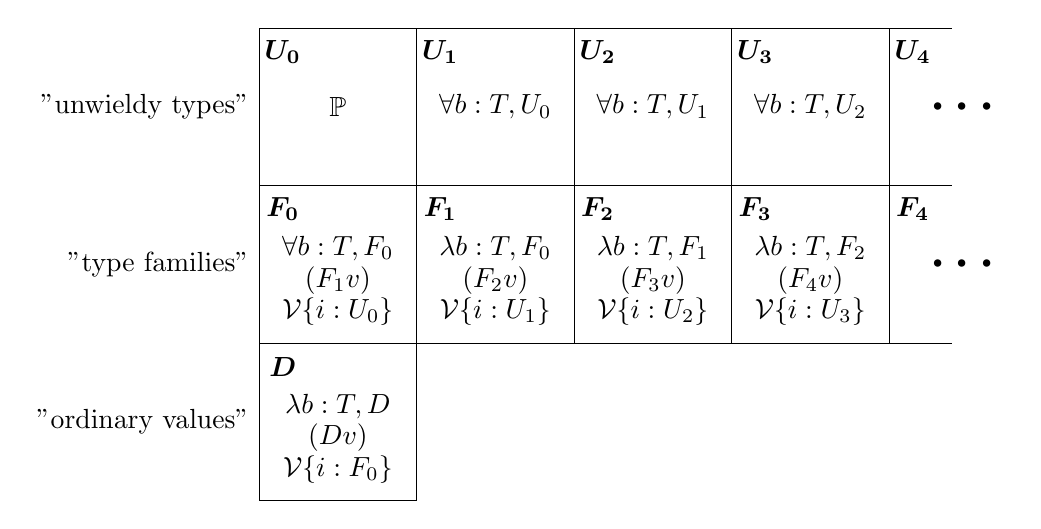
\begin{tikzpicture}
    \pgfsetxvec{\pgfpoint{2cm}{0}}
    \pgfsetyvec{\pgfpoint{0}{-2cm}}

    \draw (0,0.5) node[left]{"unwieldy types"};
    \draw (0,1.5) node[left]{"type families"};
    \draw (0,2.5) node[left]{"ordinary values"};
    \foreach \y in {0,1,2} {
      \draw (0,\y) rectangle (1,\y+1);
      \draw (4,\y) -- (4.4,\y);
    }
    \foreach \y in {0,1} {
      \draw (4.2,\y+0.5) node[right]{{\LARGE \boldmath $\cdots$}};
    }
    \foreach \x in {0,1,2,3,4} {
      \draw (\x+0.15,0.15) node[]{{\boldmath $U_\x$}};
      \draw (\x+0.15,1.15) node[]{{\boldmath $F_\x$}};
    }
    \foreach \x in {0,1,2,3} {
      \draw (\x+0.5,1.8) node[]{$\usageKnown{U_\x}{i}$};
    }
    \draw (0.15,2.15) node[]{{\boldmath $D$}};
    \draw (0.5,0.5) node[]{$\Prop$};
    \draw (0.5,1.4) node[]{$\forall b:T,F_0$};
    \draw (0.5,1.6) node[]{$(F_1 v)$};
    \draw (0.5,2.4) node[]{$\lambda b:T,D$};
    \draw (0.5,2.6) node[]{$(D v)$};
    \draw (0.5,2.8) node[]{$\usageKnown{F_0}{i}$};
    \foreach \l/\x/\r in {0/1/2,1/2/3,2/3/4} {
%      \pgfmathsetmacro{\l}{\x-1};
      \draw (\x,0) rectangle (\x+1,1);
      \draw (\x+0.5,0.5) node[]{$\forall b:T,U_{\l}$};
      \draw (\x,1) rectangle (\x+1,2);
      \draw (\x+0.5,1.4) node[]{$\lambda b:T,F_{\l}$};
      \draw (\x+0.5,1.6) node[]{$(F_{\r} v)$};
    }
  \end{tikzpicture}

  \vspace{0.5cm}

  In the above chart, $V:T$ denotes a variable-usage-site whose bound type is in the cell $T$. The literal $T$ can denote any \emph{type}, and $v$ can denote any \emph{value}, which we shall define forthwith. The other letters refer to cells; for example, $F_2$ can denote any formula from the cell $F_2$.

  If\footnote{In general, it may be very difficult to determine whether a formula has a type \emph{at all}. But it is easy (again, $O(n)$) to give any formula $V$ a \emph{provisional} type $T$, where if $V$ has any types at all, its types are exactly all the well-typed beta-conversions of $T$. The only difficult part is determining whether function arguments have the correct types.} a formula has a type, that type is in the cell directly above its own. Thus, the \emph{values} (formulas that can be members of types) include everything except the top row, and the \emph{types} (formulas that can have members) include everything except the bottom-most cells. As such, $F_0$ (the cell of propositions) is the unique cell whose formulas are both types and values.
\end{document}
